% !TEX TS-program = pdflatex
% !TEX root = ../LightMicroRep.tex

%************************************************
\chapter{Light Sheet Microscopy}
\label{chp:Lightsheet}
%************************************************
%\numberwithin{figure}{section}
%----------------------------------------------------------------------------------------
%	INTRODUCTION
%----------------------------------------------------------------------------------------

\section{Introduction}

\paragraph{Aim} To study the features of Light Sheet Microscopy method in image acquisition.
\\

Light sheet microscopy is a technique to achieve high resolution optical sectioning and named so to reflect the mode of illumination in which a sheet of light illuminates plane(s) in the sample. 
This mode of illumination coming from the side of detection ensures signal arises only from in-focus regions and reduces exposure of other areas \cite{Power2017}. 
The comparison of this mode of plane illumination to the point illumination in confocal laser scanning microscopy (LSM) is shown in Fig.~\ref{fig:lsccomp}. 

\begin{figure}[h!]
\begin{minipage}[b]{0.55\textwidth}
\centering
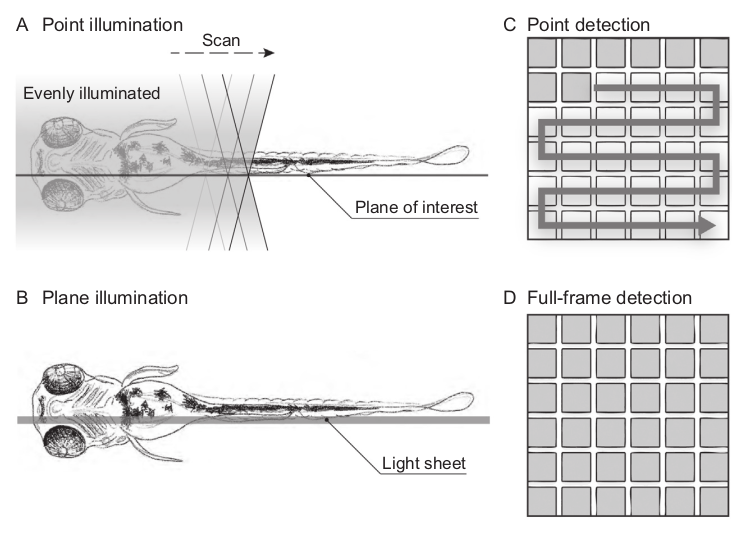
\includegraphics[width=\columnwidth]{Exp_1_Lightsheet/Figures/lightsheetconcomp}
\caption{Comparison of point illumination in conventional confocal technique and plane illumination in light sheet microscopy (from Weber et al \cite{Weber2014}).}
\label{fig:lsccomp}
\end{minipage}\hfill
\begin{minipage}[b]{0.4\textwidth}
\centering
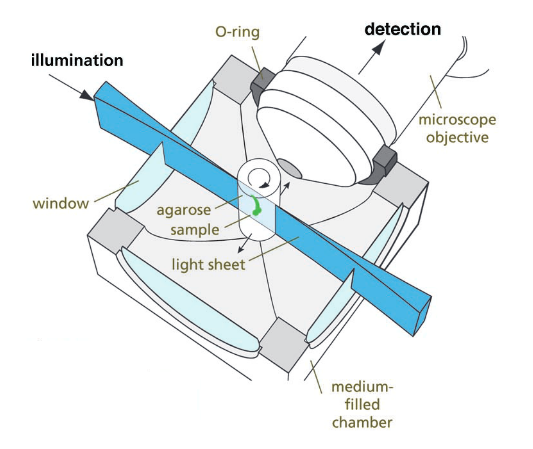
\includegraphics[width=\columnwidth]{Exp_1_Lightsheet/Figures/LSscheme2}
\caption{Schematic of light sheet microscopy (adapted from Huisken et al \cite{Huisken2004}).}
\label{fig:lsscheme}
\end{minipage}
\end{figure}

The advantage of plane illumination is immediate, namely only a specific plane being illuminated, in contrast to LSM where a significant part of the specimen being illuminated, even when imaging only a single plane (Fig.~\ref{fig:lsccomp}~A\&B). 
Furthermore, the detection mode in LSM where the laser is scanned across the plane for image acquisition is disadvantageous in respect to acquisition time in comparison to light sheet that allows the whole frame to be acquired at once (Fig.~\ref{fig:lsccomp}~C\&D).

%----------------------------------------------------------------------------------------
%	METHODS
%----------------------------------------------------------------------------------------

\section{Methods}

The device used for this experiment is a horizontal microscope Zeiss Lightsheet.Z1 with temperature regulated sample chamber and filled with medium (water). 
The detection is orthogonal against the illumination plane (Fig. \ref{fig:lsscheme}.) 

The specimen is put into a capillary filled with low melting agarose and then placed in the chamber. 
The sample is then positioned to face the imaging lens at an angle (to minimize light path through agarose). 
Fluorescence excitation is by blue laser (488 nm), and images are recorded at 16 bits.

The samples in this experiment are the autofluorescent \textit{Eleocharis acicularis} and \textit{Egeria densa} (\textit{Elodea}).

%----------------------------------------------------------------------------------------
%	RESULTS AND DISCUSSION
%----------------------------------------------------------------------------------------
\section{Results and Discussion}

The obtained maximum intensity projection of both samples are presented in Fig.~\ref{fig:EEmip}. 
Due to the advantage of Light Sheet Microscopy, imaging was done relatively quick as a full frame of a z-stack could be obtained almost instantly as compared to other high resolution methods, chiefly LSM. 

\begin{figure}[h!]
\centering
\subfloat[\textit{\textit{E. acicularis}}\label{eleomip}]{\includegraphics[width=.45\columnwidth]{Exp_1_Lightsheet/Figures/EleoMIP_30um}}\hspace{0.1mm}
\subfloat[\textit{Elodea}\label{elodmip}]{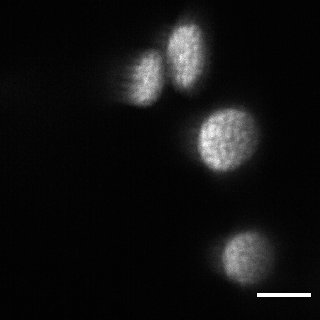
\includegraphics[width=.45\columnwidth]{Exp_1_Lightsheet/Figures/ElodMIP_5um}}\\
\caption{Maximum intensity projections of \textit{E. acicularis} and \textit{Elodea} specimen. 
Objective lens: Plan Apochromat 20$\times$/1.0 UV Vis for both images. 
Scalebar is 30 $\mu$m on A and 5 $\mu$m on B.}
\label{fig:EEmip}
\end{figure}

The fact that illumination comes in a certain direction (either left or right) means that some structure could stand as a hindrance that casts a ``shadow'' that would obscure another structure behind it from being properly illuminated. 
For this, the device allows the option to ``pivot'' the sample called the \textit{Pivot Scan} that moves the sample slightly (in a rotating motion) to minimize this shadowing effect. 
This can be seen by comparing the images presented in Fig.~\ref{nopiv} \& Fig.~\ref{piv} where structures can be obscured by shadows and pivoting the sample slightly could minimize the effect and allows a back-positioned structures to be illuminated and observed as well.

In this image (Fig.~\ref{fig:Elepiv}) some stripping artifacts could be also observed. 
These artifacts is the result of features that scatter or absorb the light resulting in weaker illumination, visible as stripes. 
A solution for this is by obtaining several z-stacks at different angles. 
Then a composite of these z-stacks can be created using algorithms. 
However this would increase acquisition time dramatically and exposes the sample to a higher amount of illumination \cite{NikonLS}. 

The two illumination sources (from the left and right side of the sample) aim to ensure that both sides of the sample can be evenly exposed to illumination, to deal with the fact that if the illumination comes only from one side, e.g. left, the far side of the sample (right) would be exposed to less amount of illumination in comparison to the near side. 
The use of dual illumination should in theory reduce the stripping artifacts, however not significantly enough in this case. 

\begin{figure}[h!]
\centering
\subfloat[No Pivot\label{nopiv}]{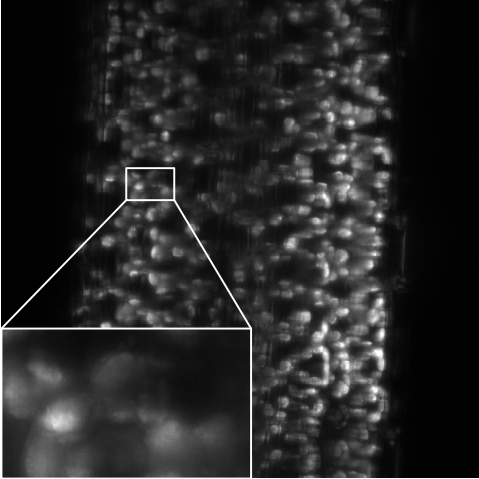
\includegraphics[width=.45\columnwidth]{Exp_1_Lightsheet/Figures/Eleo}}\hspace{.1mm}
\subfloat[Pivot\label{piv}]{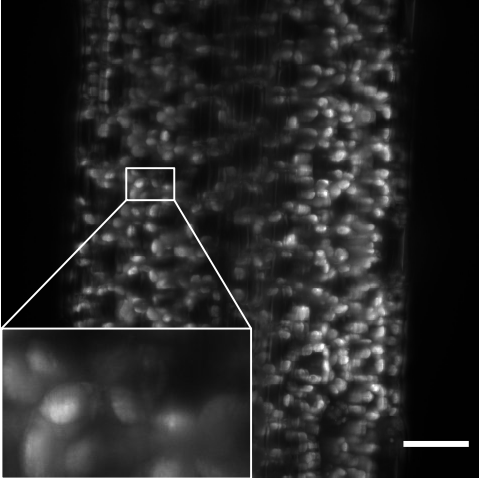
\includegraphics[width=.45\columnwidth]{Exp_1_Lightsheet/Figures/Eleopiv_30um}}\\
\caption{Pivot scan comparison of \textit{E. acicularis}. 
Inset shows an example of where the illumination of a structure is hindered by another structure in front of it and pivoting the sample minimize this effect. 
Objective lens: Plan Apochromat 20$\times$/1.0 UV Vis. 
Scalebar is 30 $\mu$m.}
\label{fig:Elepiv}
\end{figure}

Light sheet microscopy also minimizes photodamage due to the reduction of exposure in other areas and hence suitable to image live cells, along with the fact that the device is equipped with other support systems (e.g. temperature regulation). 
A time series image was recorded in which the chloroplast of \textit{Elodea} could be observed moving around in Fig.~\ref{fig:Elomov}. 
\\
\begin{figure}[h]
\centering
\subfloat[]{\animategraphics[loop,autoplay,width=.24\columnwidth]{8}{Exp_1_Lightsheet/Figures/Elo_tf_animov5um3/frame-}{0}{9}}\hspace{0.1mm}
\subfloat[]{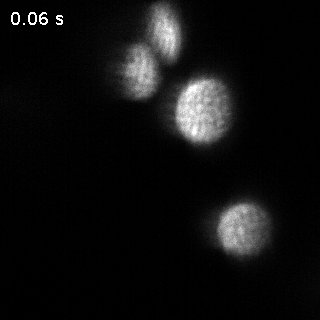
\includegraphics[width=.24\columnwidth]{Exp_1_Lightsheet/Figures/Elo_tf_animov5um3/frame-3}}\hspace{0.1mm}
\subfloat[]{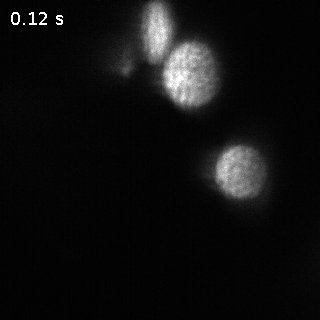
\includegraphics[width=.24\columnwidth]{Exp_1_Lightsheet/Figures/Elo_tf_animov5um3/frame-6}}\hspace{0.1mm}
\subfloat[]{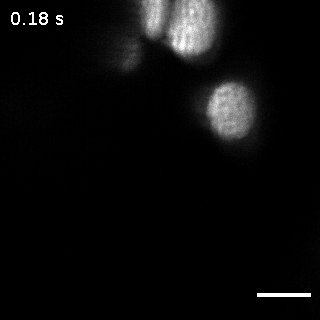
\includegraphics[width=.24\columnwidth]{Exp_1_Lightsheet/Figures/Elo_tf_animov5um3_scbar/frame-9}}
\caption{Movement of chloroplast in \textit{Elodea} captured in 10 frames (t: 0.00-0.18 s). 
\textbf{A} is animated (Best viewed on Adobe Acrobat Reader, for other pdf-reader, please follow this \href{https://i.imgur.com/MbgWUVP.mp4}{link to an external webpage} or alternatively, open the accompanying animated file.), \textbf{B}-\textbf{D} show some selected frames. 
Scalebar is 5$\mu$m.} 
%webpage: https://imgur.com/a/VyLE9jk
\label{fig:Elomov}
\end{figure}

%----------------------------------------------------------------------------------------
%	BIBLIOGRAPHY
%----------------------------------------------------------------------------------------

\renewcommand{\refname}{\spacedlowsmallcaps{References}} % For modifying the bibliography heading

%\bibliographystyle{unsrt}

%\bibliography{literature.bib} % The file containing the bibliography

%----------------------------------------------------------------------------------------
